\documentclass[11pt,a4paper]{article}
\usepackage[utf8]{inputenc}
\usepackage[T1]{fontenc}
\usepackage{geometry}
\usepackage{graphicx}
\usepackage{fancyhdr}
\usepackage{longtable}
\usepackage{booktabs}
\usepackage{xcolor}
\usepackage{hyperref}
\usepackage{lastpage}
\usepackage{enumitem}
\usepackage{tikz}
\usetikzlibrary{shapes,arrows,positioning}

\geometry{margin=1in}

\definecolor{nis2blue}{RGB}{0,51,153}
\definecolor{nis2gray}{RGB}{100,100,100}
\definecolor{nis2red}{RGB}{204,0,0}
\definecolor{nis2orange}{RGB}{255,153,0}
\definecolor{nis2yellow}{RGB}{255,204,0}
\definecolor{nis2green}{RGB}{0,153,51}

\pagestyle{fancy}
\fancyhf{}
\fancyhead[L]{\textcolor{nis2blue}{\textbf{Incident Response Plan}}}
\fancyhead[R]{\includegraphics[height=0.8cm]{logo.png}}
\fancyfoot[L]{\textcolor{nis2gray}{\small \jobname}}
\fancyfoot[C]{\textcolor{nis2gray}{\small \textbf{CONFIDENTIAL}}}
\fancyfoot[R]{\textcolor{nis2gray}{\small Page \thepage\ of \pageref{LastPage}}}

\renewcommand{\headrulewidth}{2pt}
\renewcommand{\footrulewidth}{1pt}

\hypersetup{
    colorlinks=true,
    linkcolor=nis2blue,
    filecolor=nis2blue,
    urlcolor=nis2blue,
}

\begin{document}

\begin{titlepage}
    \centering
    \vspace*{2cm}

    {\Huge\bfseries\textcolor{nis2blue}{Incident Response Plan}\par}
    \vspace{0.5cm}
    {\Large NIS2 Directive Compliance\par}
    \vspace{2cm}

    {\Large\textbf{Organization:} [ORGANIZATION]\par}
    \vspace{0.5cm}
    {\Large\textbf{Effective Date:} \today\par}
    \vspace{0.5cm}
    {\Large\textbf{Version:} 1.0\par}
    \vspace{2cm}

    {\large\textbf{Classification:} \textcolor{nis2red}{CONFIDENTIAL}\par}
    \vfill

    {\large Incident Response Team Leader: [NAME]\par}
    {\large Emergency Contact: [PHONE NUMBER]\par}
    {\large Email: [INCIDENT EMAIL]\par}
    \vspace{1cm}

    {\small NIS2 Directive (EU) 2022/2555 Article 23 Compliance\par}
\end{titlepage}

\tableofcontents
\newpage

\section{Document Control}

\begin{table}[h]
\centering
\begin{tabular}{|l|l|}
\hline
\textbf{Document Title} & Incident Response Plan \\
\hline
\textbf{Document Owner} & Chief Information Security Officer \\
\hline
\textbf{Version} & 1.0 \\
\hline
\textbf{Effective Date} & \today \\
\hline
\textbf{Review Frequency} & Semi-Annual \\
\hline
\textbf{Next Review Date} & [DATE] \\
\hline
\end{tabular}
\caption{Document Control Information}
\end{table}

\section{Executive Summary}

This Incident Response Plan (IRP) provides a structured approach to managing cybersecurity incidents in compliance with NIS2 Directive requirements. The plan ensures rapid detection, containment, eradication, and recovery from security incidents while meeting regulatory reporting obligations.

\subsection{Key Objectives}
\begin{itemize}
    \item Minimize impact of security incidents on business operations
    \item Ensure timely detection and response to incidents
    \item Comply with NIS2 incident reporting requirements
    \item Preserve evidence for investigations
    \item Learn from incidents to improve security posture
\end{itemize}

\section{Incident Response Team}

\subsection{Team Structure}

\begin{table}[h]
\centering
\begin{tabular}{|p{4cm}|p{4cm}|p{4cm}|}
\hline
\textbf{Role} & \textbf{Name} & \textbf{Contact} \\
\hline
IR Team Leader & [Name] & [Phone/Email] \\
\hline
CISO & [Name] & [Phone/Email] \\
\hline
IT Manager & [Name] & [Phone/Email] \\
\hline
Security Analyst & [Name] & [Phone/Email] \\
\hline
Legal Counsel & [Name] & [Phone/Email] \\
\hline
Communications Lead & [Name] & [Phone/Email] \\
\hline
External Forensics & [Company] & [Phone/Email] \\
\hline
\end{tabular}
\caption{Incident Response Team Contacts}
\end{table}

\subsection{Team Responsibilities}

\subsubsection{IR Team Leader}
\begin{itemize}
    \item Overall incident coordination
    \item Escalation decisions
    \item Communication with management
    \item Resource allocation
\end{itemize}

\subsubsection{Security Analysts}
\begin{itemize}
    \item Incident detection and triage
    \item Technical analysis and investigation
    \item Evidence collection
    \item Containment actions
\end{itemize}

\subsubsection{Legal Counsel}
\begin{itemize}
    \item Legal implications assessment
    \item Regulatory reporting guidance
    \item Evidence handling procedures
    \item External communication review
\end{itemize}

\section{Incident Classification}

\subsection{Severity Levels}

\begin{table}[h]
\centering
\begin{tabular}{|l|p{10cm}|}
\hline
\rowcolor{nis2red} \textcolor{white}{\textbf{Critical}} &
\textcolor{white}{Complete service disruption, data breach affecting sensitive data, ransomware encryption of critical systems, nation-state attack} \\
\hline
\rowcolor{nis2orange} \textbf{High} &
Major service degradation, unauthorized access to critical systems, malware on multiple systems, successful phishing campaign \\
\hline
\rowcolor{nis2yellow} \textbf{Medium} &
Limited service impact, attempted unauthorized access, isolated malware infection, minor data exposure \\
\hline
\rowcolor{nis2green} \textbf{Low} &
No service impact, failed attack attempts, policy violations, suspicious activity \\
\hline
\end{tabular}
\caption{Incident Severity Classification}
\end{table}

\subsection{NIS2 Significant Incidents}

A significant incident under NIS2 has caused or is capable of causing:
\begin{itemize}
    \item Severe operational disruption of services or financial loss
    \item Considerable material or non-material damage to natural or legal persons
\end{itemize}

Significant incidents require reporting to competent authorities.

\section{Incident Response Process}

\subsection{Incident Response Lifecycle}

\begin{center}
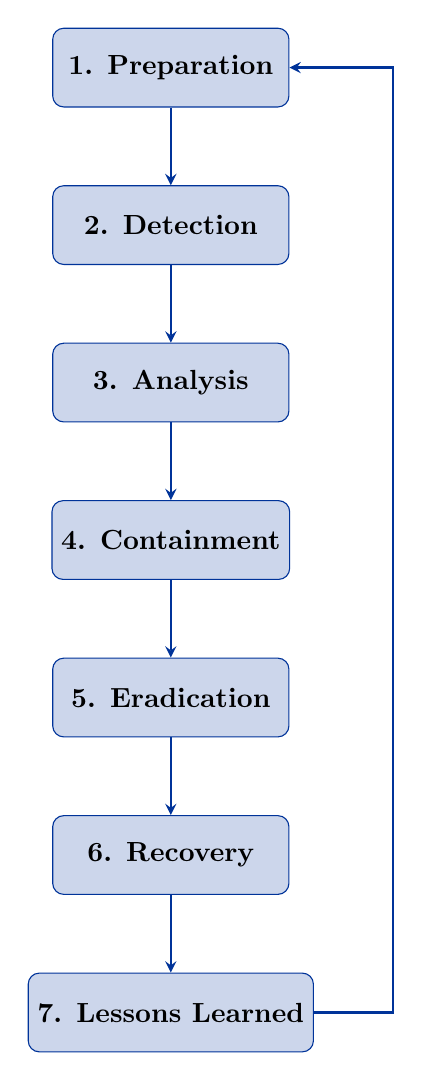
\begin{tikzpicture}[node distance=2cm, auto]
    \tikzstyle{phase} = [rectangle, rounded corners, minimum width=3cm, minimum height=1cm, text centered, draw=nis2blue, fill=nis2blue!20, font=\bfseries]
    \tikzstyle{arrow} = [thick,->,>=stealth,nis2blue]

    \node (prep) [phase] {1. Preparation};
    \node (detect) [phase, below of=prep] {2. Detection};
    \node (analysis) [phase, below of=detect] {3. Analysis};
    \node (contain) [phase, below of=analysis] {4. Containment};
    \node (eradicate) [phase, below of=contain] {5. Eradication};
    \node (recover) [phase, below of=eradicate] {6. Recovery};
    \node (lessons) [phase, below of=recover] {7. Lessons Learned};

    \draw [arrow] (prep) -- (detect);
    \draw [arrow] (detect) -- (analysis);
    \draw [arrow] (analysis) -- (contain);
    \draw [arrow] (contain) -- (eradicate);
    \draw [arrow] (eradicate) -- (recover);
    \draw [arrow] (recover) -- (lessons);
    \draw [arrow] (lessons.east) -- ++(1,0) |- (prep.east);
\end{tikzpicture}
\end{center}

\subsection{Phase 1: Preparation}

\textbf{Ongoing Activities:}
\begin{itemize}
    \item Maintain incident response capabilities
    \item Conduct regular IR drills and tabletop exercises
    \item Update contact lists and escalation procedures
    \item Maintain incident response tools and access
    \item Train staff on incident reporting procedures
\end{itemize}

\subsection{Phase 2: Detection and Identification}

\textbf{Detection Sources:}
\begin{itemize}
    \item Security monitoring tools (SIEM, IDS/IPS)
    \item Automated alerts
    \item User reports
    \item External notifications (customers, partners, authorities)
    \item Threat intelligence
\end{itemize}

\textbf{Actions:}
\begin{enumerate}
    \item Receive and log incident report
    \item Assign incident ID and open ticket
    \item Perform initial triage
    \item Notify IR Team Leader
\end{enumerate}

\textbf{Timeline:} Immediate (within 15 minutes of detection)

\subsection{Phase 3: Analysis and Scoping}

\textbf{Actions:}
\begin{enumerate}
    \item Gather additional information
    \item Determine incident type and scope
    \item Assess impact and severity
    \item Identify affected systems and data
    \item Determine root cause
    \item Document findings
\end{enumerate}

\textbf{Timeline:} 1-4 hours depending on complexity

\textbf{Key Questions:}
\begin{itemize}
    \item What systems are affected?
    \item What data is at risk?
    \item How did the incident occur?
    \item Is the threat still active?
    \item What is the business impact?
\end{itemize}

\subsection{Phase 4: Containment}

\subsubsection{Short-term Containment}
\textbf{Immediate actions to prevent incident spread:}
\begin{itemize}
    \item Isolate affected systems from network
    \item Disable compromised accounts
    \item Block malicious IP addresses
    \item Implement temporary access restrictions
\end{itemize}

\subsubsection{Long-term Containment}
\textbf{Sustained measures while preparing for recovery:}
\begin{itemize}
    \item Apply temporary patches or workarounds
    \item Implement enhanced monitoring
    \item Restore services to temporary infrastructure
    \item Continue evidence collection
\end{itemize}

\textbf{Timeline:} Critical incidents - within 1 hour; High - within 4 hours

\subsection{Phase 5: Eradication}

\textbf{Actions:}
\begin{enumerate}
    \item Remove malware and backdoors
    \item Delete unauthorized accounts
    \item Close vulnerabilities exploited
    \item Reset compromised credentials
    \item Apply security patches
    \item Rebuild compromised systems if necessary
\end{enumerate}

\textbf{Verification:}
\begin{itemize}
    \item Scan systems for remaining threats
    \item Verify vulnerability remediation
    \item Confirm no persistence mechanisms remain
\end{itemize}

\subsection{Phase 6: Recovery}

\textbf{Actions:}
\begin{enumerate}
    \item Restore systems from clean backups
    \item Verify system integrity
    \item Implement additional security controls
    \item Gradually return systems to production
    \item Monitor for signs of reinfection
    \item Validate business functionality
\end{enumerate}

\textbf{Recovery Priorities:}
\begin{enumerate}
    \item Critical business systems (RTO < 4 hours)
    \item Essential services (RTO < 24 hours)
    \item Standard systems (RTO < 72 hours)
\end{enumerate}

\subsection{Phase 7: Post-Incident Activities}

\textbf{Lessons Learned Meeting:}
\begin{itemize}
    \item Conduct within 2 weeks of incident closure
    \item Review incident timeline and response
    \item Identify what worked well
    \item Document areas for improvement
    \item Update procedures and controls
\end{itemize}

\textbf{Final Report Components:}
\begin{itemize}
    \item Executive summary
    \item Incident timeline
    \item Root cause analysis
    \item Impact assessment
    \item Response effectiveness
    \item Recommendations
    \item Action items
\end{itemize}

\section{NIS2 Incident Reporting}

\subsection{Reporting Timeline}

\begin{longtable}{|p{3cm}|p{4cm}|p{6cm}|}
\hline
\textbf{Timeframe} & \textbf{Report Type} & \textbf{Content} \\
\hline
\endfirsthead
\hline
\textbf{Timeframe} & \textbf{Report Type} & \textbf{Content} \\
\hline
\endhead
\textbf{24 hours} & Early Warning & Basic notification of significant incident \\
\hline
\textbf{72 hours} & Incident Notification & Initial assessment: type, severity, impact, indicators of compromise \\
\hline
\textbf{1 month} & Final Report & Detailed analysis, root cause, impacts, response actions, preventive measures \\
\hline
\caption{NIS2 Incident Reporting Timeline}
\end{longtable}

\subsection{Reporting Authority}

\textbf{Competent Authority:} [NATIONAL CSIRT/COMPETENT AUTHORITY]

\textbf{Contact Information:}
\begin{itemize}
    \item Email: [AUTHORITY EMAIL]
    \item Phone: [AUTHORITY PHONE]
    \item Portal: [REPORTING PORTAL URL]
\end{itemize}

\subsection{Report Content Requirements}

\subsubsection{Early Warning (24 hours)}
\begin{itemize}
    \item Incident detected: Date and time
    \item Incident type (e.g., ransomware, data breach, DDoS)
    \item Preliminary impact assessment
    \item Contact person details
\end{itemize}

\subsubsection{Incident Notification (72 hours)}
\begin{itemize}
    \item Incident description and classification
    \item Affected systems and services
    \item Estimated number of affected users/customers
    \item Geographic scope
    \item Indicators of compromise (IoCs)
    \item Initial assessment of severity and impact
    \item Response measures taken
\end{itemize}

\subsubsection{Final Report (1 month)}
\begin{itemize}
    \item Comprehensive incident timeline
    \item Root cause analysis
    \item Detailed impact assessment (financial, operational, reputational)
    \item Complete list of affected systems and data
    \item Response and recovery actions
    \item Lessons learned
    \item Preventive measures implemented
    \item Recommendations for the sector
\end{itemize}

\section{Communication Plan}

\subsection{Internal Communications}

\begin{table}[h]
\centering
\begin{tabular}{|l|l|l|}
\hline
\textbf{Audience} & \textbf{Information} & \textbf{Timing} \\
\hline
Management & Impact, response status & Immediate \\
\hline
Employees & Need-to-know basis & As appropriate \\
\hline
IT Staff & Technical details & Immediate \\
\hline
\end{tabular}
\caption{Internal Communication Matrix}
\end{table}

\subsection{External Communications}

\begin{itemize}
    \item \textbf{Customers:} If service impact or data exposure affects them
    \item \textbf{Partners:} If incident may affect their systems or data
    \item \textbf{Regulators:} As required by NIS2
    \item \textbf{Media:} Only through designated spokesperson
    \item \textbf{Law Enforcement:} For criminal incidents
\end{itemize}

\textbf{Communication Guidelines:}
\begin{itemize}
    \item All external communications approved by legal counsel
    \item Maintain message consistency
    \item Protect sensitive technical details
    \item Be transparent and factual
\end{itemize}

\section{Evidence Handling}

\subsection{Evidence Collection}
\begin{itemize}
    \item Maintain chain of custody documentation
    \item Use forensically sound tools and methods
    \item Create and verify cryptographic hashes
    \item Document all collection activities
    \item Store evidence securely
\end{itemize}

\subsection{Evidence Types}
\begin{itemize}
    \item System logs and event data
    \item Network traffic captures
    \item Memory dumps
    \item Disk images
    \item Screenshots and photographs
    \item Email and communication records
\end{itemize}

\section{Incident Response Tools}

\subsection{Technical Tools}
\begin{itemize}
    \item SIEM platform
    \item Forensic analysis tools
    \item Network traffic analyzers
    \item Malware analysis sandbox
    \item Backup and recovery systems
    \item Secure communication channels
\end{itemize}

\subsection{Documentation Templates}
\begin{itemize}
    \item Incident Report Form
    \item Evidence Collection Log
    \item Chain of Custody Form
    \item Communication Templates
    \item Lessons Learned Template
\end{itemize}

\section{Testing and Exercises}

\subsection{Tabletop Exercises}
\begin{itemize}
    \item Frequency: Quarterly
    \item Participants: IR Team and key stakeholders
    \item Scenarios: Based on current threat landscape
    \item Document lessons learned
\end{itemize}

\subsection{Technical Drills}
\begin{itemize}
    \item Frequency: Semi-annually
    \item Test technical response procedures
    \item Validate tools and access
    \item Measure response times
\end{itemize}

\subsection{Full-scale Simulations}
\begin{itemize}
    \item Frequency: Annually
    \item Comprehensive incident simulation
    \item Include all stakeholders
    \item Test communications and escalation
\end{itemize}

\section{Plan Maintenance}

This plan shall be reviewed and updated:
\begin{itemize}
    \item Semi-annually at minimum
    \item After significant incidents
    \item After exercises reveal gaps
    \item When organizational or technical changes occur
    \item When regulatory requirements change
\end{itemize}

\section{Appendices}

\subsection{Appendix A: Incident Report Form}
[Include incident report template]

\subsection{Appendix B: Contact Lists}
[Detailed contact information for all stakeholders]

\subsection{Appendix C: Incident Playbooks}
[Specific procedures for common incident types:
\begin{itemize}
    \item Ransomware Response
    \item Data Breach Response
    \item DDoS Response
    \item Insider Threat Response
\end{itemize}]

\subsection{Appendix D: Legal and Regulatory Requirements}
[Specific reporting requirements by jurisdiction]

\section{Approval}

\begin{table}[h]
\centering
\begin{tabular}{|l|l|l|}
\hline
\textbf{Role} & \textbf{Name} & \textbf{Signature \& Date} \\
\hline
CISO & & \\
\hline
Legal Counsel & & \\
\hline
CEO & & \\
\hline
\end{tabular}
\caption{Plan Approval}
\end{table}

\end{document}
